% This LaTeX document needs to be compiled with XeLaTeX.
\documentclass[10pt]{article}
\usepackage[utf8]{inputenc}
\usepackage{ucharclasses}
\usepackage{hyperref}
\hypersetup{colorlinks=true, linkcolor=blue, filecolor=magenta, urlcolor=cyan,}
\urlstyle{same}
\usepackage{amsmath}
\usepackage{amsfonts}
\usepackage{amssymb}
\usepackage[version=4]{mhchem}
\usepackage{stmaryrd}
\usepackage{bbold}
\usepackage{graphicx}
\usepackage[export]{adjustbox}
\graphicspath{ {./images/} }
\usepackage{multirow}
\usepackage{polyglossia}
\usepackage{fontspec}
\setmainlanguage{english}
\setotherlanguages{hindi, spanish}
\IfFontExistsTF{Noto Serif Devanagari}
{\newfontfamily\hindifont{Noto Serif Devanagari}}
{\IfFontExistsTF{Kohinoor Devanagari}
  {\newfontfamily\hindifont{Kohinoor Devanagari}}
  {\IfFontExistsTF{Devanagari MT}
    {\newfontfamily\hindifont{Devanagari MT}}
    {\IfFontExistsTF{Lohit Devanagari}
      {\newfontfamily\hindifont{Lohit Devanagari}}
      {\IfFontExistsTF{FreeSerif}
        {\newfontfamily\hindifont{FreeSerif}}
        {\newfontfamily\hindifont{Arial Unicode MS}}
}}}}
\IfFontExistsTF{CMU Serif}
{\newfontfamily\lgcfont{CMU Serif}}
{\IfFontExistsTF{DejaVu Sans}
  {\newfontfamily\lgcfont{DejaVu Sans}}
  {\newfontfamily\lgcfont{Georgia}}
}
\setDefaultTransitions{\lgcfont}{}
\setTransitionsForDevanagari{\hindifont}{\rmfamily}

\begin{document}
© International Baccalaureate Organization 2023

All rights reserved. No part of this product may be reproduced in any form or by any electronic or mechanical means, including information storage and retrieval systems, without the prior written permission from the IB. Additionally, the license tied with this product prohibits use of any selected files or extracts from this product. Use by third parties, including but not limited to publishers, private teachers, tutoring or study services, preparatory schools, vendors operating curriculum mapping services or teacher resource digital platforms and app developers, whether fee-covered or not, is prohibited and is a criminal offense.

More information on how to request written permission in the form of a license can be obtained from \href{https://ibo.org/become-an-ib-school/ib-publishing/licensing/applying-for-alicense/}{https://ibo.org/become-an-ib-school/ib-publishing/licensing/applying-for-alicense/}.\\
© Organisation du Baccalauréat International 2023

Tous droits réservés. Aucune partie de ce produit ne peut être reproduite sous quelque forme ni par quelque moyen que ce soit, électronique ou mécanique, y compris des systèmes de stockage et de récupération d'informations, sans l'autorisation écrite préalable de l'IB. De plus, la licence associée à ce produit interdit toute utilisation de tout fichier ou extrait sélectionné dans ce produit. L'utilisation par des tiers, y compris, sans toutefois s'y limiter, des éditeurs, des professeurs particuliers, des services de tutorat ou d'aide aux études, des établissements de préparation à l'enseignement supérieur, des fournisseurs de services de planification des programmes d'études, des gestionnaires de plateformes pédagogiques en ligne, et des développeurs d'applications, moyennant paiement ou non, est interdite et constitue une infraction pénale.

Pour plus d'informations sur la procédure à suivre pour obtenir une autorisation écrite sous la forme d'une licence, rendez-vous à l'adresse \href{https://ibo.org/become-an-ib-school/}{https://ibo.org/become-an-ib-school/} ib-publishing/licensing/applying-for-a-license/.\\
© Organización del Bachillerato Internacional, 2023

Todos los derechos reservados. No se podrá reproducir ninguna parte de este producto de ninguna forma ni por ningún medio electrónico o mecánico, incluidos los sistemas de almacenamiento y recuperación de información, sin la previa autorización por escrito del IB. Además, la licencia vinculada a este producto prohíbe el uso de todo archivo o fragmento seleccionado de este producto. El uso por parte de terceros -lo que incluye, a título enunciativo, editoriales, profesores particulares, servicios de apoyo académico o ayuda para el estudio, colegios preparatorios, desarrolladores de aplicaciones y entidades que presten servicios de planificación curricular u ofrezcan recursos para docentes mediante plataformas digitales-, ya sea incluido en tasas o no, está prohibido y constituye un delito.

En este enlace encontrará más información sobre cómo solicitar una autorización por escrito en forma de licencia: \href{https://ibo.org/become-an-ib-school/ib-publishing/licensing/}{https://ibo.org/become-an-ib-school/ib-publishing/licensing/} applying-for-a-license/.

\section*{Mathematics: applications and interpretation Standard level \\
 Paper 1}
8 May 2023\\
Zone A afternoon | Zone B morning | Zone C afternoon

1 hour 30 minutes

Candidate session number

\begin{center}
\begin{tabular}{|l|l|l|l|l|l|l|l|l|l|}
\hline
 &  &  &  &  &  &  &  &  &  \\
\hline
\end{tabular}
\end{center}

\section*{Instructions to candidates}
\begin{itemize}
  \item Write your session number in the boxes above.
  \item Do not open this examination paper until instructed to do so.
  \item A graphic display calculator is required for this paper.
  \item Answer all questions.
  \item Answers must be written within the answer boxes provided.
  \item Unless otherwise stated in the question, all numerical answers should be given exactly or correct to three significant figures.
  \item A clean copy of the mathematics: applications and interpretation formula booklet is required for this paper.
  \item The maximum mark for this examination paper is [80 marks].
\end{itemize}

Answers must be written within the answer boxes provided. Full marks are not necessarily awarded for a correct answer with no working. Answers must be supported by working and/or explanations. Solutions found from a graphic display calculator should be supported by suitable working. For example, if graphs are used to find a solution, you should sketch these as part of your answer. Where an answer is incorrect, some marks may be given for a correct method, provided this is shown by written working. You are therefore advised to show all working.

\begin{enumerate}
  \item \hspace{0pt} [Maximum mark: 5]
\end{enumerate}

Zaha is designing a bridge to cross a river. She believes that the weight of the steel needed for this bridge is approximately 53632000 kg .

The exact weight of the steel needed for the bridge is 55625000 kg .\\
(a) Find the percentage error in Zaha's approximation.

Zaha's design is used to build five identical bridges.\\
(b) (i) Find the weight of the steel needed for these five bridges, to three significant figures.\\
(ii) Write down your answer to part (b)(i) in the form $a \times 10^{k}$, where $1 \leq a<10$, $k \in \mathbb{Z}$.\\[0pt]
2. [Maximum mark: 6]

Angel has $\$ 520$ in his savings account. Angel considers investing the money for 5 years with a bank. The bank offers an annual interest rate of $1.2 \%$ compounded quarterly.\\
(a) Calculate the amount of money Angel would have at the end of 5 years with the bank. Give your answer correct to two decimal places.

Instead of investing the money, Angel decides to buy a phone that costs $\$ 520$. At the end of 5 years, the phone will have a value of $\$ 30$. It may be assumed that the depreciation rate per year is constant.\\
(b) Calculate the annual depreciation rate of the phone.\\[0pt]
3. [Maximum mark: 7]

In a school, 200 students solved a problem in a mathematics competition. Their times to solve the problem were recorded and the following cumulative frequency graph was produced.\\
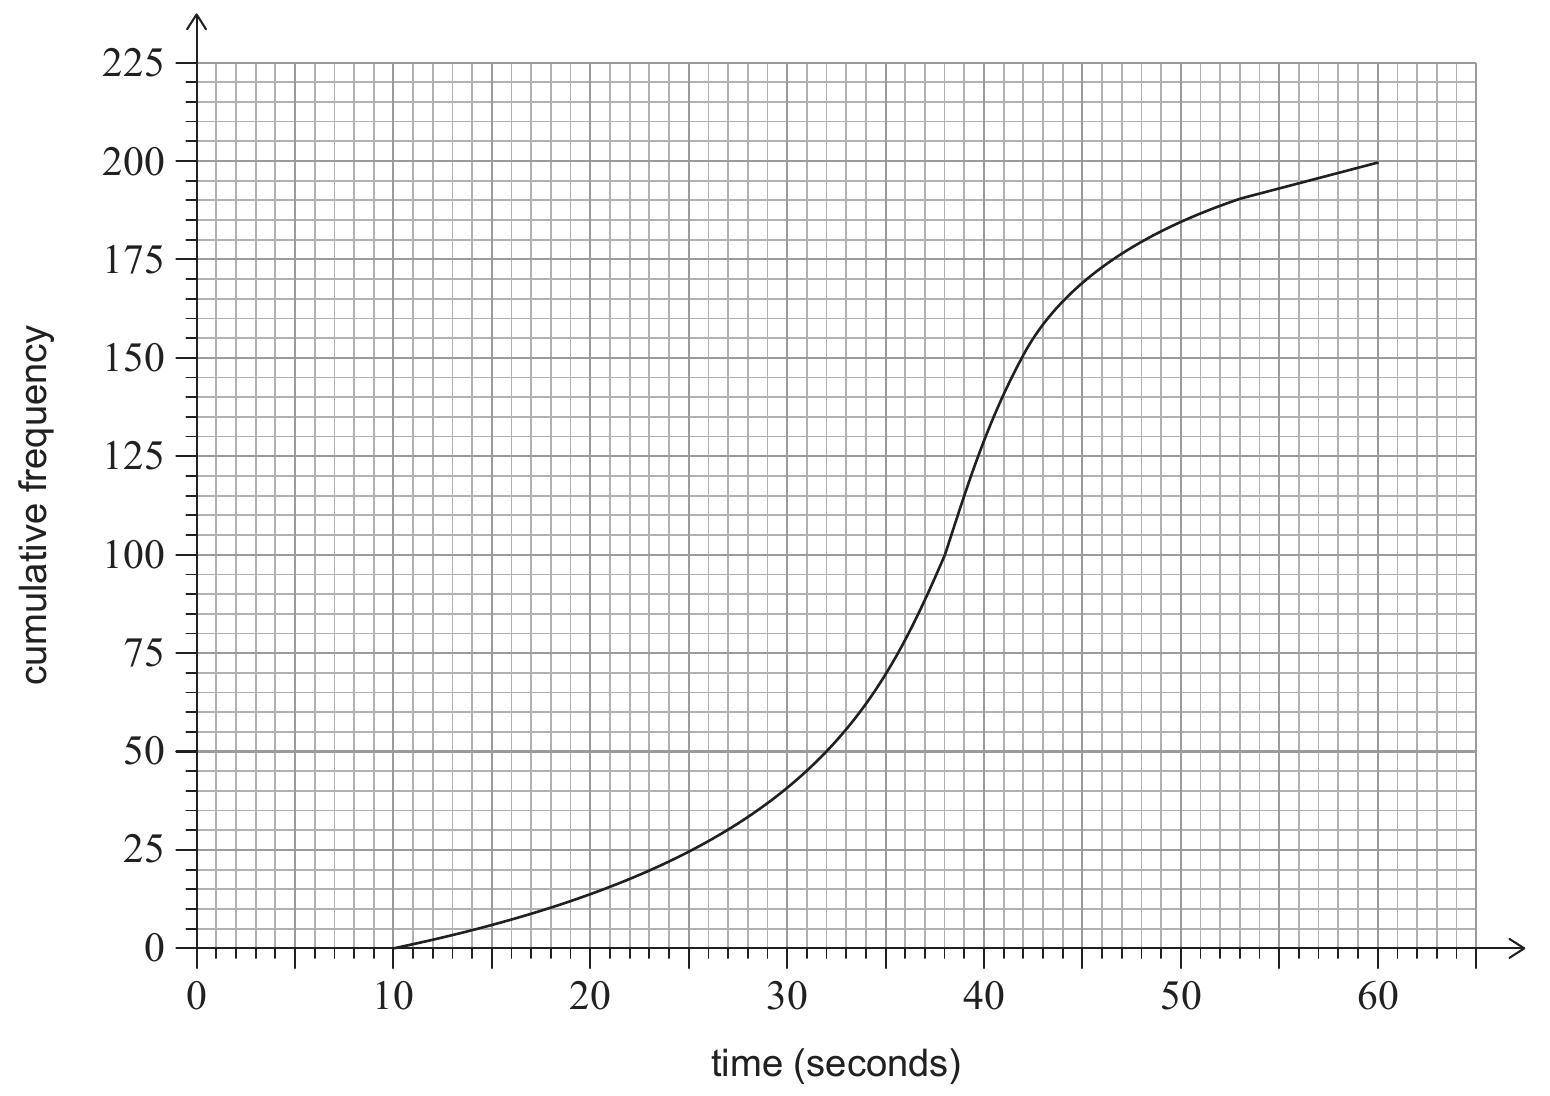
\includegraphics[max width=\textwidth, center]{4108bb7b-f3e3-487f-89c2-57a89f48fc01-05}\\
(a) Use the graph to find\\
(i) the median time;\\
(ii) the lower quartile;\\
(iii) the upper quartile;\\
(iv) the interquartile range.

Cedric took 14 seconds to solve the problem.\\
(b) Determine whether Cedric's time is an outlier.\\
(This question continues on the following page)\\
(Question 3 continued)\\[0pt]
4. [Maximum mark: 6]

At a running club, Sung-Jin conducts a test to determine if there is any association between an athlete's age and their best time taken to run 100 m . Eight athletes are chosen at random, and their details are shown below.

\begin{center}
\begin{tabular}{|c|c|c|c|c|c|c|c|c|}
\hline
Athlete & A & B & C & D & E & F & G & H \\
\hline
Age (years) & 13 & 17 & 22 & 18 & 19 & 25 & 11 & 36 \\
\hline
Time (seconds) & 13.4 & 14.6 & 13.4 & 12.9 & 12.0 & 11.8 & 17.0 & 13.1 \\
\hline
\end{tabular}
\end{center}

Sung-Jin decides to calculate the Spearman's rank correlation coefficient for his set of data.\\
(a) Complete the table of ranks.

\begin{center}
\begin{tabular}{|l|l|l|l|l|l|l|l|l|}
\hline
Athlete & A & B & C & D & E & F & G & H \\
\hline
Age rank &  &  & 3 &  &  &  &  &  \\
\hline
Time rank &  &  &  &  &  &  & 1 &  \\
\hline
\end{tabular}
\end{center}

(b) Calculate the Spearman's rank correlation coefficient, $r_{s}$.\\
(c) Interpret this value of $r_{s}$ in the context of the question.\\
(d) Suggest a mathematical reason why Sung-Jin may have decided not to use Pearson's product-moment correlation coefficient with his data from the original table.\\[0pt]
5. [Maximum mark: 4]

The following frequency distribution table shows the test grades for a group of students.

\begin{center}
\begin{tabular}{|c|c|c|c|c|c|c|c|}
\hline
Grade & 1 & 2 & 3 & 4 & 5 & 6 & 7 \\
\hline
Frequency & 1 & 4 & 7 & 9 & $p$ & 9 & 4 \\
\hline
\end{tabular}
\end{center}

For this distribution, the mean grade is 4.5 .\\
(a) Write down the total number of students in terms of $p$.\\
(b) Calculate the value of $p$.\\[0pt]
6. [Maximum mark: 6]

A company that owns many restaurants wants to determine if there are differences in the quality of the food cooked for three different meals: breakfast, lunch and dinner.

Their quality assurance team randomly selects 500 items of food to inspect. The quality of this food is classified as perfect, satisfactory, or poor. The data is summarized in the following table.

\begin{center}
\begin{tabular}{|l|l|l|l|l|l|}
\hline
\multicolumn{2}{|c|}{\multirow{2}{*}{}} & \multicolumn{3}{|c|}{Quality} &  \\
\hline
 &  & Perfect & Satisfactory & Poor & Total \\
\hline
\multirow{3}{*}{Meal} & Breakfast & 101 & 124 & 7 & 232 \\
\hline
 & Lunch & 68 & 81 & 5 & 154 \\
\hline
 & Dinner & 35 & 69 & 10 & 114 \\
\hline
 & Total & 204 & 274 & 22 & 500 \\
\hline
\end{tabular}
\end{center}

An item of food is chosen at random from these 500 .\\
(a) Find the probability that its quality is not perfect, given that it is from breakfast.

A $\chi^{2}$ test at the $5 \%$ significance level is carried out to determine if there is significant evidence of a difference in the quality of the food cooked for the three meals.

The critical value for this test is 9.488 .

The hypotheses for this test are:\\
$\mathrm{H}_{0}$ : The quality of the food and the type of meal are independent.\\
$\mathrm{H}_{1}$ : The quality of the food and the type of meal are not independent.\\
(b) Find the $\chi^{2}$ statistic.\\
(c) State, with justification, the conclusion for this test.\\
(This question continues on the following page)\\
(Question 6 continued)\\[0pt]
7. [Maximum mark: 6]

Ani owns four cafes represented by points $\mathrm{A}, \mathrm{B}, \mathrm{C}$ and D . Ani wants to divide the area into delivery regions. This process has been started in the following incomplete Voronoi diagram, where 1 unit represents 1 kilometre.\\
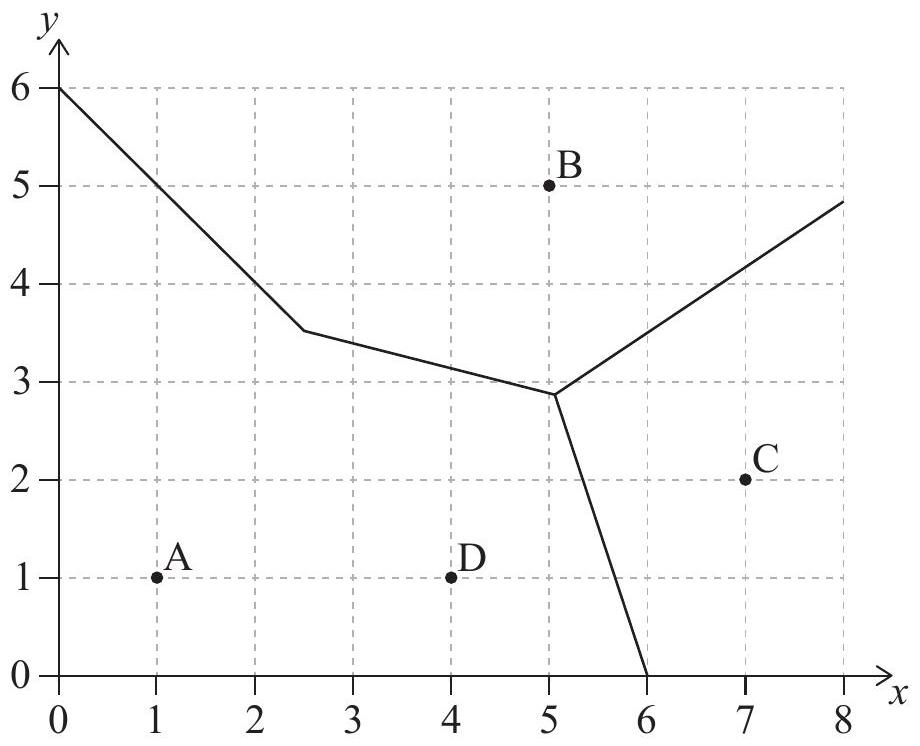
\includegraphics[max width=\textwidth, center]{4108bb7b-f3e3-487f-89c2-57a89f48fc01-11}

The midpoint of CD is (5.5, 1.5).\\[0pt]
(a) Show that the equation of the perpendicular bisector of [CD] is $y=-3 x+18$.\\
(b) Complete the Voronoi diagram shown above.

Ani opens an office equidistant from three of the cafes, $\mathrm{B}, \mathrm{C}$ and D . The equation of the perpendicular bisector of $[\mathrm{BC}]$ is $3 y=2 x-1.5$.\\
(c) Find the coordinates of the office.\\
(This question continues on the following page)\\
(Question 7 continued)\\[0pt]
8. [Maximum mark: 5]

Ruhi buys a scoop of ice cream in the shape of a sphere with a radius of 3.4 cm . The ice cream is served in a cone, and it may be assumed that $\frac{1}{5}$ of the volume of the ice cream is inside the cone. This is shown in the following diagram.\\
diagram not to scale\\
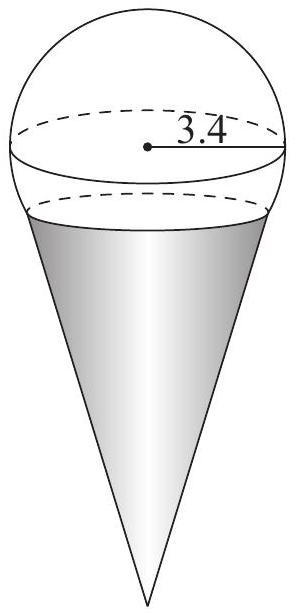
\includegraphics[max width=\textwidth, center]{4108bb7b-f3e3-487f-89c2-57a89f48fc01-13}\\
(a) Calculate the volume of ice cream that is not inside the cone.

The cone has a slant height of 11 cm and a radius of 3 cm .\\
The outside of the cone is covered with chocolate.\\
(b) Calculate the surface area of the cone that is covered with chocolate. Give your answer correct to the nearest $\mathrm{cm}^{2}$.\\[0pt]
9. [Maximum mark: 6]

The lengths of the seeds from a particular mango tree are approximated by a normal distribution with a mean of 4 cm and a standard deviation of 0.25 cm .

A seed from this mango tree is chosen at random.\\
(a) Calculate the probability that the length of the seed is less than 3.7 cm .

It is known that $30 \%$ of the seeds have a length greater than $k \mathrm{~cm}$.\\
(b) Find the value of $k$.

For a seed of length $d \mathrm{~cm}$, chosen at random, $\mathrm{P}(4-m<d<4+m)=0.6$.\\
(c) Find the value of $m$.\\[0pt]
10. [Maximum mark: 8]

A player throws a basketball. The height of the basketball is modelled by

$$
h(t)=-4.75 t^{2}+8.75 t+1.5, t \geq 0
$$

where $h$ is the height of the basketball above the ground, in metres, and $t$ is the time, in seconds, after it was thrown.\\
(a) Find how long it takes for the basketball to reach its maximum height.\\
(b) Assuming that no player catches the basketball, find how long it would take for the basketball to hit the ground.

Another player catches the basketball when it is at a height of 1.2 metres.\\
(c) Find the value of $t$ when this player catches the basketball.\\
(d) Write down two limitations of using $h(t)$ to model the height of the basketball.\\[0pt]
11. [Maximum mark: 7]

Consider $f(x)=3 x^{2}-\frac{5}{x}, x \neq 0$. The graph of $f$ for $0<x \leq 5$ is shown on the following axes.\\
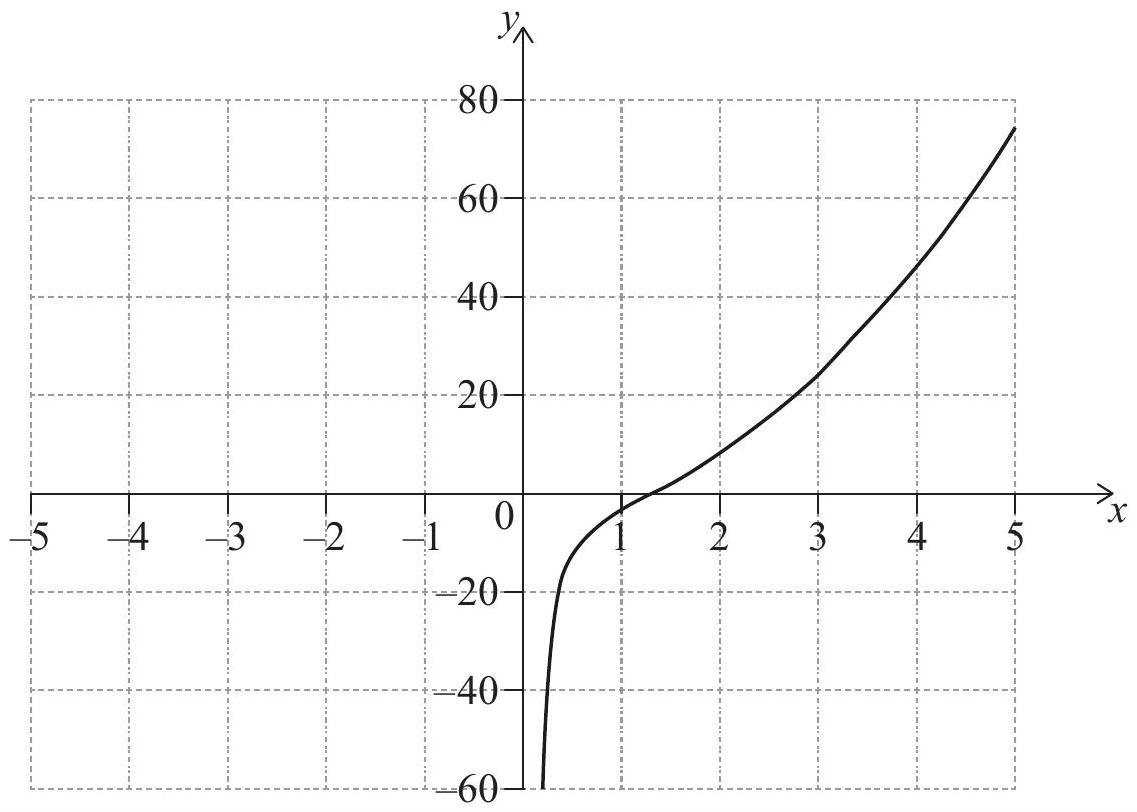
\includegraphics[max width=\textwidth, center]{4108bb7b-f3e3-487f-89c2-57a89f48fc01-16}\\
(a) (i) Sketch the graph of $f$, for $-5 \leq x<0$, on the same axes.\\
(ii) Write down the $x$-coordinate of the local minimum point.\\
(b) Use your graphic display calculator to find the solutions to the equation $f(x)=20$.\\
(c) Write down the equation of the vertical asymptote for the graph of $f$.\\
$\_\_\_\_$\\
$\_\_\_\_$\\
$\_\_\_\_$\\
$\_\_\_\_$\\
$\_\_\_\_$\\
$\_\_\_\_$\\
$\_\_\_\_$\\
$\_\_\_\_$\\
$\_\_\_\_$\\
$\_\_\_\_$\\
$\_\_\_\_$\\
$\_\_\_\_$\\
$\_\_\_\_$

\section*{Please do not write on this page.}
Answers written on this page will not be marked.\\[0pt]
12. [Maximum mark: 5]

In a game, balls are thrown to hit a target. The random variable $X$ is the number of times the target is hit in five attempts. The probability distribution for $X$ is shown in the following table.

\begin{center}
\begin{tabular}{|c|c|c|c|c|c|c|}
\hline
$\boldsymbol{x}$ & 0 & 1 & 2 & 3 & 4 & 5 \\
\hline
$\mathbf{P}(\boldsymbol{X}=\boldsymbol{x})$ & 0.15 & 0.2 & $k$ & 0.16 & $2 k$ & 0.25 \\
\hline
\end{tabular}
\end{center}

(a) Find the value of $k$.

The player has a chance to win money based on how many times they hit the target.

The gain for the player, in $\$$, is shown in the following table, where a negative gain means that the player loses money.

\begin{center}
\begin{tabular}{|c|c|c|c|c|c|c|}
\hline
$\boldsymbol{x}$ & 0 & 1 & 2 & 3 & 4 & 5 \\
\hline
Player's gain (\$) & -4 & -3 & -1 & 0 & 1 & 4 \\
\hline
\end{tabular}
\end{center}

(b) Determine whether this game is fair. Justify your answer.\\[0pt]
13. [Maximum mark: 9]

An engineer wants to calculate the cross-sectional area of a dam. The cross-section of the dam can be modelled by a curve and two straight lines as shown in the following diagram, where distances are measured in metres.\\
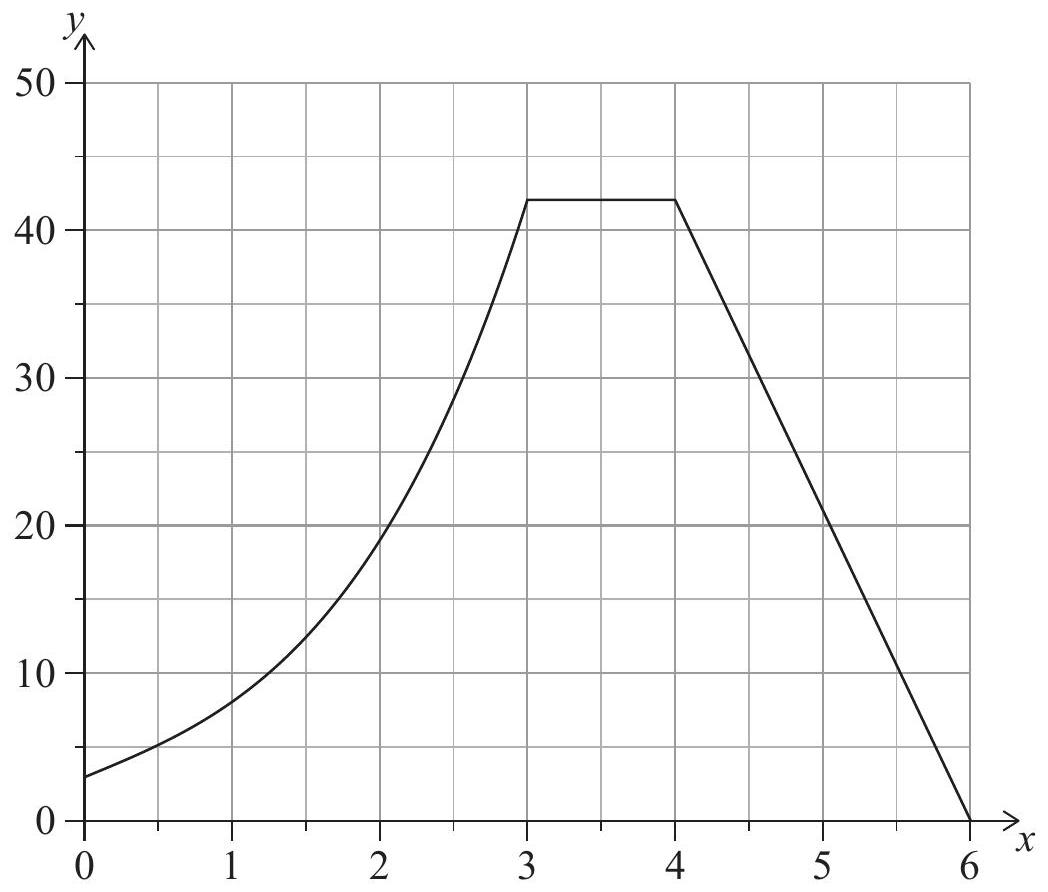
\includegraphics[max width=\textwidth, center]{4108bb7b-f3e3-487f-89c2-57a89f48fc01-19}

The curve is modelled by a function $f(x)$. The following table gives values of $f(x)$ for different values of $x$ in the interval $0 \leq x \leq 3$.

\begin{center}
\begin{tabular}{|c|r|r|r|r|r|r|r|}
\hline
$\boldsymbol{x}$ & 0 & 0.5 & 1 & 1.5 & 2 & 2.5 & 3 \\
\hline
$\boldsymbol{y}=\boldsymbol{f}(\boldsymbol{x})$ & 3 & 5.13 & 8 & 12.4 & 19 & 28.6 & 42 \\
\hline
\end{tabular}
\end{center}

(a) Calculate an estimate for the area in the interval $0 \leq x \leq 3$ by using the trapezoidal rule with three equal intervals.

It is known that $f^{\prime}(x)=3 x^{2}+4$ in the domain $0<x<3$.\\
(b) Find an expression for $f(x)$, in the domain $0<x<3$.\\
(c) Hence find the actual area of the entire cross-section.\\
(This question continues on the following page)\\
(Question 13 continued)

\section*{References:}
© International Baccalaureate Organization 2023

\section*{Please do not write on this page.}
Answers written on this page will not be marked.


\end{document}